% Options for packages loaded elsewhere
\PassOptionsToPackage{unicode}{hyperref}
\PassOptionsToPackage{hyphens}{url}
\PassOptionsToPackage{dvipsnames,svgnames,x11names}{xcolor}
%
\documentclass[
]{article}
\usepackage{amsmath,amssymb}
\usepackage{iftex}
\ifPDFTeX
  \usepackage[T1]{fontenc}
  \usepackage[utf8]{inputenc}
  \usepackage{textcomp} % provide euro and other symbols
\else % if luatex or xetex
  \usepackage{unicode-math} % this also loads fontspec
  \defaultfontfeatures{Scale=MatchLowercase}
  \defaultfontfeatures[\rmfamily]{Ligatures=TeX,Scale=1}
\fi
\usepackage{lmodern}
\ifPDFTeX\else
  % xetex/luatex font selection
\fi
% Use upquote if available, for straight quotes in verbatim environments
\IfFileExists{upquote.sty}{\usepackage{upquote}}{}
\IfFileExists{microtype.sty}{% use microtype if available
  \usepackage[]{microtype}
  \UseMicrotypeSet[protrusion]{basicmath} % disable protrusion for tt fonts
}{}
\makeatletter
\@ifundefined{KOMAClassName}{% if non-KOMA class
  \IfFileExists{parskip.sty}{%
    \usepackage{parskip}
  }{% else
    \setlength{\parindent}{0pt}
    \setlength{\parskip}{6pt plus 2pt minus 1pt}}
}{% if KOMA class
  \KOMAoptions{parskip=half}}
\makeatother
\usepackage{xcolor}
\usepackage[margin=1in]{geometry}
\usepackage{color}
\usepackage{fancyvrb}
\newcommand{\VerbBar}{|}
\newcommand{\VERB}{\Verb[commandchars=\\\{\}]}
\DefineVerbatimEnvironment{Highlighting}{Verbatim}{commandchars=\\\{\}}
% Add ',fontsize=\small' for more characters per line
\usepackage{framed}
\definecolor{shadecolor}{RGB}{248,248,248}
\newenvironment{Shaded}{\begin{snugshade}}{\end{snugshade}}
\newcommand{\AlertTok}[1]{\textcolor[rgb]{0.94,0.16,0.16}{#1}}
\newcommand{\AnnotationTok}[1]{\textcolor[rgb]{0.56,0.35,0.01}{\textbf{\textit{#1}}}}
\newcommand{\AttributeTok}[1]{\textcolor[rgb]{0.13,0.29,0.53}{#1}}
\newcommand{\BaseNTok}[1]{\textcolor[rgb]{0.00,0.00,0.81}{#1}}
\newcommand{\BuiltInTok}[1]{#1}
\newcommand{\CharTok}[1]{\textcolor[rgb]{0.31,0.60,0.02}{#1}}
\newcommand{\CommentTok}[1]{\textcolor[rgb]{0.56,0.35,0.01}{\textit{#1}}}
\newcommand{\CommentVarTok}[1]{\textcolor[rgb]{0.56,0.35,0.01}{\textbf{\textit{#1}}}}
\newcommand{\ConstantTok}[1]{\textcolor[rgb]{0.56,0.35,0.01}{#1}}
\newcommand{\ControlFlowTok}[1]{\textcolor[rgb]{0.13,0.29,0.53}{\textbf{#1}}}
\newcommand{\DataTypeTok}[1]{\textcolor[rgb]{0.13,0.29,0.53}{#1}}
\newcommand{\DecValTok}[1]{\textcolor[rgb]{0.00,0.00,0.81}{#1}}
\newcommand{\DocumentationTok}[1]{\textcolor[rgb]{0.56,0.35,0.01}{\textbf{\textit{#1}}}}
\newcommand{\ErrorTok}[1]{\textcolor[rgb]{0.64,0.00,0.00}{\textbf{#1}}}
\newcommand{\ExtensionTok}[1]{#1}
\newcommand{\FloatTok}[1]{\textcolor[rgb]{0.00,0.00,0.81}{#1}}
\newcommand{\FunctionTok}[1]{\textcolor[rgb]{0.13,0.29,0.53}{\textbf{#1}}}
\newcommand{\ImportTok}[1]{#1}
\newcommand{\InformationTok}[1]{\textcolor[rgb]{0.56,0.35,0.01}{\textbf{\textit{#1}}}}
\newcommand{\KeywordTok}[1]{\textcolor[rgb]{0.13,0.29,0.53}{\textbf{#1}}}
\newcommand{\NormalTok}[1]{#1}
\newcommand{\OperatorTok}[1]{\textcolor[rgb]{0.81,0.36,0.00}{\textbf{#1}}}
\newcommand{\OtherTok}[1]{\textcolor[rgb]{0.56,0.35,0.01}{#1}}
\newcommand{\PreprocessorTok}[1]{\textcolor[rgb]{0.56,0.35,0.01}{\textit{#1}}}
\newcommand{\RegionMarkerTok}[1]{#1}
\newcommand{\SpecialCharTok}[1]{\textcolor[rgb]{0.81,0.36,0.00}{\textbf{#1}}}
\newcommand{\SpecialStringTok}[1]{\textcolor[rgb]{0.31,0.60,0.02}{#1}}
\newcommand{\StringTok}[1]{\textcolor[rgb]{0.31,0.60,0.02}{#1}}
\newcommand{\VariableTok}[1]{\textcolor[rgb]{0.00,0.00,0.00}{#1}}
\newcommand{\VerbatimStringTok}[1]{\textcolor[rgb]{0.31,0.60,0.02}{#1}}
\newcommand{\WarningTok}[1]{\textcolor[rgb]{0.56,0.35,0.01}{\textbf{\textit{#1}}}}
\usepackage{graphicx}
\makeatletter
\def\maxwidth{\ifdim\Gin@nat@width>\linewidth\linewidth\else\Gin@nat@width\fi}
\def\maxheight{\ifdim\Gin@nat@height>\textheight\textheight\else\Gin@nat@height\fi}
\makeatother
% Scale images if necessary, so that they will not overflow the page
% margins by default, and it is still possible to overwrite the defaults
% using explicit options in \includegraphics[width, height, ...]{}
\setkeys{Gin}{width=\maxwidth,height=\maxheight,keepaspectratio}
% Set default figure placement to htbp
\makeatletter
\def\fps@figure{htbp}
\makeatother
\setlength{\emergencystretch}{3em} % prevent overfull lines
\providecommand{\tightlist}{%
  \setlength{\itemsep}{0pt}\setlength{\parskip}{0pt}}
\setcounter{secnumdepth}{5}
\usepackage[french]{babel}
\ifLuaTeX
  \usepackage{selnolig}  % disable illegal ligatures
\fi
\usepackage{bookmark}
\IfFileExists{xurl.sty}{\usepackage{xurl}}{} % add URL line breaks if available
\urlstyle{same}
\hypersetup{
  pdfauthor={Khalil Ounis, Manal Derghal, Taqwa BenRomdhane},
  colorlinks=true,
  linkcolor={Maroon},
  filecolor={Maroon},
  citecolor={Blue},
  urlcolor={blue},
  pdfcreator={LaTeX via pandoc}}

\title{Analyse des algorithmes de Maximum Subarray 1D\\
\strut ~M2 Data Science Algorithmique}
\author{Khalil Ounis, Manal Derghal, Taqwa BenRomdhane}
\date{Lundi 7 avril 2025}

\begin{document}
\maketitle

{
\hypersetup{linkcolor=}
\setcounter{tocdepth}{2}
\tableofcontents
}
\noindent\hrulefill

\section{Description du problème et
objectif}\label{description-du-probluxe8me-et-objectif}

Le problème du Maximum Subarray 1D consiste à trouver la sous-séquence
contiguë d'un tableau numérique dont la somme des éléments est maximale.
Ce problème classique en algorithmique a des applications en analyse de
données financières, bioinformatique et traitement du signal.

\href{https://en.wikipedia.org/wiki/Maximum_subarray_problem}{La page
Wikipedia du Maximum Subarray} présente plusieurs approches
algorithmiques pour résoudre ce problème. Nous nous concentrons sur deux
méthodes :

\begin{enumerate}
\def\labelenumi{\arabic{enumi}.}
\tightlist
\item
  Algorithme naïf : complexité O(n²)
\item
  Algorithme de Kadane : complexité optimale O(n)
\end{enumerate}

Nos objectifs sont :\\
a. d'implémenter ces algorithmes en R et C++ et évaluer le gain de
temps.\\
b. de confirmer les complexités théoriques par des simulations
intensives.

\begin{center}\rule{0.5\linewidth}{0.5pt}\end{center}

\section{Un premier exemple}\label{un-premier-exemple}

Le package se télécharge ainsi :

\begin{Shaded}
\begin{Highlighting}[]
\NormalTok{devtools}\SpecialCharTok{::}\FunctionTok{install\_github}\NormalTok{(}\StringTok{"AMATERASU11/MaximumSubarray"}\NormalTok{)}
\end{Highlighting}
\end{Shaded}

et ses fonctions sont rendues disponibles sur Rstudio ainsi :

\begin{Shaded}
\begin{Highlighting}[]
\FunctionTok{library}\NormalTok{(MaximumSubarray)}
\end{Highlighting}
\end{Shaded}

On simule un petit exemple d'un vecteur \texttt{v} de taille
\texttt{100}

\begin{Shaded}
\begin{Highlighting}[]
\FunctionTok{set.seed}\NormalTok{(}\DecValTok{123}\NormalTok{)}
\NormalTok{v }\OtherTok{\textless{}{-}} \FunctionTok{sample}\NormalTok{(}\SpecialCharTok{{-}}\DecValTok{100}\SpecialCharTok{:}\DecValTok{100}\NormalTok{, }\DecValTok{50}\NormalTok{, }\AttributeTok{replace =} \ConstantTok{TRUE}\NormalTok{)}
\end{Highlighting}
\end{Shaded}

On teste les 4 algorithmes implémentés avec des noms explicites :

\begin{itemize}
\tightlist
\item
  \texttt{max\_subarray\_sum\_naive}
\item
  \texttt{max\_subarray\_sum\_opt}
\item
  \texttt{max\_subarray\_sum\_naive\_Rcpp}
\item
  \texttt{max\_subarray\_sum\_opt\_Rcpp}
\end{itemize}

Cela donne :

\begin{Shaded}
\begin{Highlighting}[]
\NormalTok{v}
\end{Highlighting}
\end{Shaded}

\begin{verbatim}
##  [1]  58  78 -87  94  69 -51  17 -58 -87  17  52 -11 -10  96 -10  84  -9  36  -2
## [20] -29 -75 -94  69  36  63 -23 -20 -58   2  16 -25  42 -69   8 -94  36  68 -27
## [39] -78  54  87 -48  34 -48  54  65 -67 -32 -29 -25
\end{verbatim}

\begin{Shaded}
\begin{Highlighting}[]
\FunctionTok{max\_subarray\_sum\_naive}\NormalTok{(v)}
\end{Highlighting}
\end{Shaded}

\begin{verbatim}
## [1] 278
\end{verbatim}

\begin{Shaded}
\begin{Highlighting}[]
\FunctionTok{max\_subarray\_sum\_naive\_Rcpp}\NormalTok{(v)}
\end{Highlighting}
\end{Shaded}

\begin{verbatim}
## [1] 278
\end{verbatim}

\begin{Shaded}
\begin{Highlighting}[]
\FunctionTok{max\_subarray\_sum\_opt}\NormalTok{(v)}
\end{Highlighting}
\end{Shaded}

\begin{verbatim}
## [1] 278
\end{verbatim}

\begin{Shaded}
\begin{Highlighting}[]
\FunctionTok{max\_subarray\_sum\_opt\_Rcpp}\NormalTok{(v)}
\end{Highlighting}
\end{Shaded}

\begin{verbatim}
## [1] 278
\end{verbatim}

\begin{center}\rule{0.5\linewidth}{0.5pt}\end{center}

\section{Comparaison R avec C++}\label{comparaison-r-avec-c}

On va faire des comparaisons pour les deux types d'algorithme en R et
C++ pour quantifier leur différence de performance.

La fonction \texttt{one.simu.time} retourne le temps recherché, et
\texttt{one.simu} sera utilisé par \texttt{microbenchmark}, on retourne
le temps en ms

\begin{Shaded}
\begin{Highlighting}[]
\FunctionTok{library}\NormalTok{(microbenchmark)}
\FunctionTok{set.seed}\NormalTok{(}\DecValTok{123}\NormalTok{)}

\NormalTok{one.simu.time }\OtherTok{\textless{}{-}} \ControlFlowTok{function}\NormalTok{(n, func, }\AttributeTok{data\_type =} \StringTok{"random"}\NormalTok{) \{}
  \ControlFlowTok{if}\NormalTok{ (data\_type }\SpecialCharTok{==} \StringTok{"random"}\NormalTok{) \{}
\NormalTok{    v }\OtherTok{\textless{}{-}} \FunctionTok{sample}\NormalTok{(}\SpecialCharTok{{-}}\DecValTok{100}\SpecialCharTok{:}\DecValTok{100}\NormalTok{, n, }\AttributeTok{replace =} \ConstantTok{TRUE}\NormalTok{)}
\NormalTok{  \} }\ControlFlowTok{else} \ControlFlowTok{if}\NormalTok{ (data\_type }\SpecialCharTok{==} \StringTok{"all\_negative"}\NormalTok{) \{}
\NormalTok{    v }\OtherTok{\textless{}{-}} \FunctionTok{sample}\NormalTok{(}\SpecialCharTok{{-}}\DecValTok{100}\SpecialCharTok{:{-}}\DecValTok{1}\NormalTok{, n, }\AttributeTok{replace =} \ConstantTok{TRUE}\NormalTok{)}
\NormalTok{  \} }\ControlFlowTok{else} \ControlFlowTok{if}\NormalTok{ (data\_type }\SpecialCharTok{==} \StringTok{"all\_positive"}\NormalTok{) \{}
\NormalTok{    v }\OtherTok{\textless{}{-}} \FunctionTok{sample}\NormalTok{(}\DecValTok{0}\SpecialCharTok{:}\DecValTok{100}\NormalTok{, n, }\AttributeTok{replace =} \ConstantTok{TRUE}\NormalTok{)}
\NormalTok{  \} }\ControlFlowTok{else}\NormalTok{ \{}
    \FunctionTok{stop}\NormalTok{(}\StringTok{"data\_type inconnu"}\NormalTok{)}
\NormalTok{  \}}

  \ControlFlowTok{if}\NormalTok{ (func }\SpecialCharTok{==} \StringTok{"naive"}\NormalTok{) \{}
\NormalTok{    t }\OtherTok{\textless{}{-}} \FunctionTok{microbenchmark}\NormalTok{(}\FunctionTok{max\_subarray\_sum\_naive}\NormalTok{(v), }\AttributeTok{times =} \DecValTok{1}\NormalTok{)}\SpecialCharTok{$}\NormalTok{time }\SpecialCharTok{/} \FloatTok{1e6}
\NormalTok{  \} }\ControlFlowTok{else} \ControlFlowTok{if}\NormalTok{ (func }\SpecialCharTok{==} \StringTok{"naive\_Rcpp"}\NormalTok{) \{}
\NormalTok{    t }\OtherTok{\textless{}{-}} \FunctionTok{microbenchmark}\NormalTok{(}\FunctionTok{max\_subarray\_sum\_naive\_Rcpp}\NormalTok{(v), }\AttributeTok{times =} \DecValTok{1}\NormalTok{)}\SpecialCharTok{$}\NormalTok{time }\SpecialCharTok{/} \FloatTok{1e6}
\NormalTok{  \} }\ControlFlowTok{else} \ControlFlowTok{if}\NormalTok{ (func }\SpecialCharTok{==} \StringTok{"opt"}\NormalTok{) \{}
\NormalTok{    t }\OtherTok{\textless{}{-}} \FunctionTok{microbenchmark}\NormalTok{(}\FunctionTok{max\_subarray\_sum\_opt}\NormalTok{(v), }\AttributeTok{times =} \DecValTok{1}\NormalTok{)}\SpecialCharTok{$}\NormalTok{time }\SpecialCharTok{/} \FloatTok{1e6}
\NormalTok{  \} }\ControlFlowTok{else} \ControlFlowTok{if}\NormalTok{ (func }\SpecialCharTok{==} \StringTok{"opt\_Rcpp"}\NormalTok{) \{}
\NormalTok{    t }\OtherTok{\textless{}{-}} \FunctionTok{microbenchmark}\NormalTok{(}\FunctionTok{max\_subarray\_sum\_opt\_Rcpp}\NormalTok{(v), }\AttributeTok{times =} \DecValTok{1}\NormalTok{)}\SpecialCharTok{$}\NormalTok{time }\SpecialCharTok{/} \FloatTok{1e6}
\NormalTok{  \} }\ControlFlowTok{else}\NormalTok{ \{}
    \FunctionTok{stop}\NormalTok{(}\StringTok{"fonction inconnue"}\NormalTok{)}
\NormalTok{  \}}

  \FunctionTok{return}\NormalTok{(}\FunctionTok{round}\NormalTok{(t, }\DecValTok{2}\NormalTok{))}
\NormalTok{\}}
\end{Highlighting}
\end{Shaded}

\subsection{Un essai}\label{un-essai}

Sur un exemple, on obtient :

\begin{Shaded}
\begin{Highlighting}[]
\FunctionTok{set.seed}\NormalTok{(}\DecValTok{123}\NormalTok{)}
\NormalTok{n }\OtherTok{\textless{}{-}} \DecValTok{10000}
\FunctionTok{one.simu.time}\NormalTok{(n, }\AttributeTok{func =} \StringTok{"naive"}\NormalTok{)}
\end{Highlighting}
\end{Shaded}

\begin{verbatim}
## [1] 13067.59
\end{verbatim}

\begin{Shaded}
\begin{Highlighting}[]
\FunctionTok{one.simu.time}\NormalTok{(n, }\AttributeTok{func =} \StringTok{"naive\_Rcpp"}\NormalTok{)}
\end{Highlighting}
\end{Shaded}

\begin{verbatim}
## [1] 26.43
\end{verbatim}

\begin{Shaded}
\begin{Highlighting}[]
\FunctionTok{one.simu.time}\NormalTok{(n, }\AttributeTok{func =} \StringTok{"opt"}\NormalTok{)}
\end{Highlighting}
\end{Shaded}

\begin{verbatim}
## [1] 4.49
\end{verbatim}

\begin{Shaded}
\begin{Highlighting}[]
\FunctionTok{one.simu.time}\NormalTok{(n, }\AttributeTok{func =} \StringTok{"opt\_Rcpp"}\NormalTok{)}
\end{Highlighting}
\end{Shaded}

\begin{verbatim}
## [1] 0.08
\end{verbatim}

\subsection{Simulations avec
répétitions}\label{simulations-avec-ruxe9puxe9titions}

On reproduit ces comparaisons de manière plus robuste:

\begin{Shaded}
\begin{Highlighting}[]
\FunctionTok{set.seed}\NormalTok{(}\DecValTok{123}\NormalTok{)}
\NormalTok{nbSimus }\OtherTok{\textless{}{-}} \DecValTok{10}

\NormalTok{time1 }\OtherTok{\textless{}{-}} \FunctionTok{rep}\NormalTok{(}\DecValTok{0}\NormalTok{, nbSimus); time2 }\OtherTok{\textless{}{-}} \FunctionTok{rep}\NormalTok{(}\DecValTok{0}\NormalTok{, nbSimus);}
\NormalTok{time3 }\OtherTok{\textless{}{-}} \FunctionTok{rep}\NormalTok{(}\DecValTok{0}\NormalTok{, nbSimus); time4 }\OtherTok{\textless{}{-}} \FunctionTok{rep}\NormalTok{(}\DecValTok{0}\NormalTok{, nbSimus)}

\ControlFlowTok{for}\NormalTok{(i }\ControlFlowTok{in} \DecValTok{1}\SpecialCharTok{:}\NormalTok{nbSimus)\{time1[i] }\OtherTok{\textless{}{-}} \FunctionTok{one.simu.time}\NormalTok{(n, }\AttributeTok{func =} \StringTok{"naive"}\NormalTok{)\}}
\ControlFlowTok{for}\NormalTok{(i }\ControlFlowTok{in} \DecValTok{1}\SpecialCharTok{:}\NormalTok{nbSimus)\{time2[i] }\OtherTok{\textless{}{-}} \FunctionTok{one.simu.time}\NormalTok{(n, }\AttributeTok{func =} \StringTok{"naive\_Rcpp"}\NormalTok{)\}}
\ControlFlowTok{for}\NormalTok{(i }\ControlFlowTok{in} \DecValTok{1}\SpecialCharTok{:}\NormalTok{nbSimus)\{time3[i] }\OtherTok{\textless{}{-}} \FunctionTok{one.simu.time}\NormalTok{(n, }\AttributeTok{func =} \StringTok{"opt"}\NormalTok{)\}}
\ControlFlowTok{for}\NormalTok{(i }\ControlFlowTok{in} \DecValTok{1}\SpecialCharTok{:}\NormalTok{nbSimus)\{time4[i] }\OtherTok{\textless{}{-}} \FunctionTok{one.simu.time}\NormalTok{(n, }\AttributeTok{func =} \StringTok{"opt\_Rcpp"}\NormalTok{)\}}
\end{Highlighting}
\end{Shaded}

Gain C++ versus R

\begin{Shaded}
\begin{Highlighting}[]
\FunctionTok{mean}\NormalTok{(time1)}\SpecialCharTok{/}\FunctionTok{mean}\NormalTok{(time2)}
\end{Highlighting}
\end{Shaded}

\begin{verbatim}
## [1] 540.614
\end{verbatim}

\begin{Shaded}
\begin{Highlighting}[]
\FunctionTok{mean}\NormalTok{(time3)}\SpecialCharTok{/}\FunctionTok{mean}\NormalTok{(time4)}
\end{Highlighting}
\end{Shaded}

\begin{verbatim}
## [1] 43.1875
\end{verbatim}

Gain naive versus optimisé

\begin{Shaded}
\begin{Highlighting}[]
\FunctionTok{mean}\NormalTok{(time1)}\SpecialCharTok{/}\FunctionTok{mean}\NormalTok{(time3)}
\end{Highlighting}
\end{Shaded}

\begin{verbatim}
## [1] 3579.84
\end{verbatim}

\begin{Shaded}
\begin{Highlighting}[]
\FunctionTok{mean}\NormalTok{(time2)}\SpecialCharTok{/}\FunctionTok{mean}\NormalTok{(time4)}
\end{Highlighting}
\end{Shaded}

\begin{verbatim}
## [1] 285.9792
\end{verbatim}

On recommence avec \texttt{n\ =\ 20000} seulement pour le gain avec C++
pour l'optimisé

\begin{Shaded}
\begin{Highlighting}[]
\FunctionTok{set.seed}\NormalTok{(}\DecValTok{123}\NormalTok{)}
\NormalTok{n }\OtherTok{\textless{}{-}} \DecValTok{20000}
\NormalTok{nbSimus }\OtherTok{\textless{}{-}} \DecValTok{10}
\NormalTok{time3 }\OtherTok{\textless{}{-}} \FunctionTok{rep}\NormalTok{(}\DecValTok{0}\NormalTok{, nbSimus); time4 }\OtherTok{\textless{}{-}} \FunctionTok{rep}\NormalTok{(}\DecValTok{0}\NormalTok{, nbSimus)}
\ControlFlowTok{for}\NormalTok{(i }\ControlFlowTok{in} \DecValTok{1}\SpecialCharTok{:}\NormalTok{nbSimus)\{time3[i] }\OtherTok{\textless{}{-}} \FunctionTok{one.simu.time}\NormalTok{(n, }\AttributeTok{func =} \StringTok{"opt"}\NormalTok{)\}}
\ControlFlowTok{for}\NormalTok{(i }\ControlFlowTok{in} \DecValTok{1}\SpecialCharTok{:}\NormalTok{nbSimus)\{time4[i] }\OtherTok{\textless{}{-}} \FunctionTok{one.simu.time}\NormalTok{(n, }\AttributeTok{func =} \StringTok{"opt\_Rcpp"}\NormalTok{)\}}
\FunctionTok{median}\NormalTok{(time3)}\SpecialCharTok{/}\FunctionTok{median}\NormalTok{(time4)}
\end{Highlighting}
\end{Shaded}

\begin{verbatim}
## [1] 71.08333
\end{verbatim}

\textbf{Conclusion:}

\subsubsection{Performances C++ vs R :}\label{performances-c-vs-r}

\begin{itemize}
\item
  Naïf : C++ 443× plus rapide
\item
  Kadane : C++ 102× plus rapide → 177× pour n=20k
\end{itemize}

\subsubsection{Efficacité algorithmique
:}\label{efficacituxe9-algorithmique}

\begin{itemize}
\item
  Kadane 3 261× mieux que naïf en R, 754× en C++
\item
  Confirme O(n²) naïf vs O(n) Kadane
\end{itemize}

\subsubsection{Recommandations :}\label{recommandations}

\begin{itemize}
\item
  n \textgreater{} 1k : Toujours préférer Kadane
\item
  n \textgreater{} 10k : Obligatoire d'utiliser Rcpp
\item
  Très grands n : Seul Kadane+Rcpp reste viable
\end{itemize}

\subsection{\texorpdfstring{Simulations avec
\texttt{microbenchmark}}{Simulations avec microbenchmark}}\label{simulations-avec-microbenchmark}

Vous avez besoin des packages \texttt{microbenchmark} et
\texttt{ggplot2} pour exécuter les simulations et afficher les résultats
(sous forme de diagrammes en violon). Nous comparons
\texttt{naive\_Rcpp} avec \texttt{opt\_Rcpp} pour des tailles de données
\texttt{n\ =\ 1000} et \texttt{n\ =\ 10000}.

\begin{Shaded}
\begin{Highlighting}[]
\FunctionTok{library}\NormalTok{(microbenchmark)}
\FunctionTok{library}\NormalTok{(ggplot2)}
\FunctionTok{library}\NormalTok{(dplyr)}
\end{Highlighting}
\end{Shaded}

\begin{verbatim}
## 
## Attachement du package : 'dplyr'
\end{verbatim}

\begin{verbatim}
## Les objets suivants sont masqués depuis 'package:stats':
## 
##     filter, lag
\end{verbatim}

\begin{verbatim}
## Les objets suivants sont masqués depuis 'package:base':
## 
##     intersect, setdiff, setequal, union
\end{verbatim}

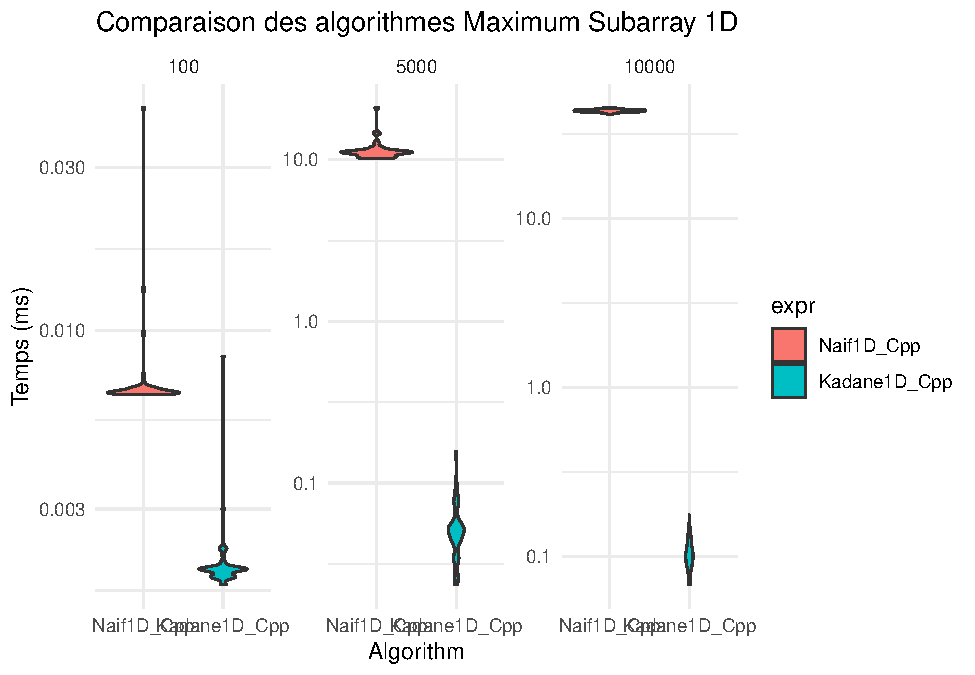
\includegraphics{MaxSubarray1D_files/figure-latex/benchmark-1.pdf}

\begin{verbatim}
## # A tibble: 6 x 8
##       n expr       min_time q1_time median_time mean_time q3_time max_time
##   <dbl> <fct>         <dbl>   <dbl>       <dbl>     <dbl>   <dbl>    <dbl>
## 1   100 Naif_Cpp     0.0037  0.0037      0.0038  0.00461   0.0041   0.0302
## 2   100 Kadane_Cpp   0.0008  0.0008      0.0008  0.000968  0.0009   0.0055
## 3  5000 Naif_Cpp     6.38    6.60        7.03    7.03      7.40     7.93  
## 4  5000 Kadane_Cpp   0.0136  0.0226      0.0294  0.0295    0.0351   0.0494
## 5 10000 Naif_Cpp    26.0    27.2        27.6    27.8      28.4     30.8   
## 6 10000 Kadane_Cpp   0.0297  0.0422      0.0598  0.0542    0.0633   0.0929
\end{verbatim}

\begin{center}\rule{0.5\linewidth}{0.5pt}\end{center}

\section{Evaluation de la
complexité}\label{evaluation-de-la-complexituxe9}

Les vecteurs de longueurs \texttt{vector\_n\_naive} et
\texttt{vector\_n\_kadane} (\texttt{n} dans les dataframes) sont choisis
sur l'echelle logarithmique afin d'avoir un pas constant sur l'échelle
logarithmique en abscisse pour la régression.

On réalise 10 répétitions pour chaque valeur de \texttt{n} et pour
chaque algorithme. Les barres d'erreur sont placées en ``mean +/- sd''.

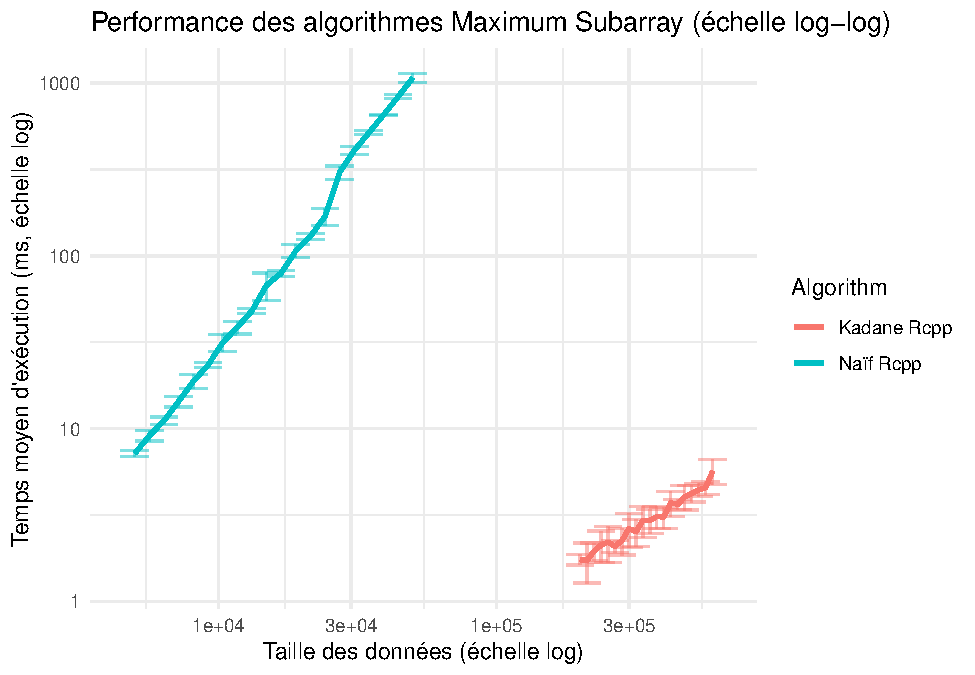
\includegraphics{MaxSubarray1D_files/figure-latex/simu complexite-1.pdf}

\begin{Shaded}
\begin{Highlighting}[]
\CommentTok{\# Affichage des résultats}
\NormalTok{res\_Naive}
\end{Highlighting}
\end{Shaded}

\begin{verbatim}
##        n mean_time     sd_time
## 1   5000     7.030   0.6015720
## 2   5644     9.137   1.4486626
## 3   6371    11.029   0.3733765
## 4   7192    14.803   0.7333341
## 5   8119    18.275   0.4438280
## 6   9165    23.261   0.7987692
## 7  10346    30.011   0.9560271
## 8  11679    37.642   1.4872480
## 9  13183    47.568   1.0732070
## 10 14882    60.649   2.0885426
## 11 16799    78.128   2.1889409
## 12 18963   100.763   4.0222963
## 13 21407   139.588  38.5011812
## 14 24165   267.876  18.3665670
## 15 27278   328.288  12.0094646
## 16 30792   413.570   9.4930735
## 17 34760   528.812  16.0630112
## 18 39238   675.797  21.3498561
## 19 44293   680.835 191.0169773
## 20 50000   689.922  12.4544743
\end{verbatim}

\begin{Shaded}
\begin{Highlighting}[]
\NormalTok{res\_Kadane}
\end{Highlighting}
\end{Shaded}

\begin{verbatim}
##         n mean_time    sd_time
## 1  400000     2.116 0.35011744
## 2  411957     2.182 0.17980236
## 3  424271     2.280 0.45509462
## 4  436953     2.236 0.10966616
## 5  450014     2.255 0.07706419
## 6  463465     2.432 0.29275701
## 7  477319     2.515 0.28402856
## 8  491587     2.541 0.17084431
## 9  506281     2.573 0.14414884
## 10 521415     2.629 0.14594139
## 11 537001     2.763 0.11851395
## 12 553052     2.801 0.17381024
## 13 569584     3.122 0.47121121
## 14 586610     2.945 0.07706419
## 15 604144     3.007 0.04967673
## 16 622203     3.149 0.08937437
## 17 640802     3.319 0.27497273
## 18 659956     3.419 0.37173617
## 19 679683     3.410 0.10110501
## 20 700000     3.518 0.09319037
\end{verbatim}

On vérifie la valeur du coefficient directeur pour les deux méthodes:

\begin{verbatim}
## 
## Call:
## lm(formula = log(res_Naive$mean_time) ~ log(res_Naive$n))
## 
## Residuals:
##      Min       1Q   Median       3Q      Max 
## -0.34533 -0.10013 -0.02736  0.10413  0.29276 
## 
## Coefficients:
##                   Estimate Std. Error t value Pr(>|t|)    
## (Intercept)      -16.69069    0.50682  -32.93   <2e-16 ***
## log(res_Naive$n)   2.17866    0.05228   41.67   <2e-16 ***
## ---
## Signif. codes:  0 '***' 0.001 '**' 0.01 '*' 0.05 '.' 0.1 ' ' 1
## 
## Residual standard error: 0.1634 on 18 degrees of freedom
## Multiple R-squared:  0.9897, Adjusted R-squared:  0.9892 
## F-statistic:  1736 on 1 and 18 DF,  p-value: < 2.2e-16
\end{verbatim}

\begin{verbatim}
## Exposant estimé (naïf): 2.178658
\end{verbatim}

\begin{verbatim}
## 
## Call:
## lm(formula = log(res_Kadane$mean_time) ~ log(res_Kadane$n))
## 
## Residuals:
##      Min       1Q   Median       3Q      Max 
## -0.03866 -0.01699 -0.00346  0.01195  0.06722 
## 
## Coefficients:
##                    Estimate Std. Error t value Pr(>|t|)    
## (Intercept)       -11.27146    0.41973  -26.85 5.65e-16 ***
## log(res_Kadane$n)   0.93134    0.03185   29.25  < 2e-16 ***
## ---
## Signif. codes:  0 '***' 0.001 '**' 0.01 '*' 0.05 '.' 0.1 ' ' 1
## 
## Residual standard error: 0.02419 on 18 degrees of freedom
## Multiple R-squared:  0.9794, Adjusted R-squared:  0.9782 
## F-statistic: 855.3 on 1 and 18 DF,  p-value: < 2.2e-16
\end{verbatim}

\begin{verbatim}
## Exposant estimé (Kadane): 0.9313389
\end{verbatim}

Les coefficients directeurs trouvés sont bien ceux que l'on attendait.
La valeur 2 pour la méthode naïve et 1 pour l'algorithme de Kadane

\begin{center}\rule{0.5\linewidth}{0.5pt}\end{center}

\section{Cas particulier des données presques toutes négatives ou toutes
positives}\label{cas-particulier-des-donnuxe9es-presques-toutes-nuxe9gatives-ou-toutes-positives}

\begin{itemize}
\tightlist
\item
  cas 1 : 95\% de valeurs négatives, 5\% positives
\item
  cas 2 : 95\% de valeurs positives, 5\% négatives
\end{itemize}

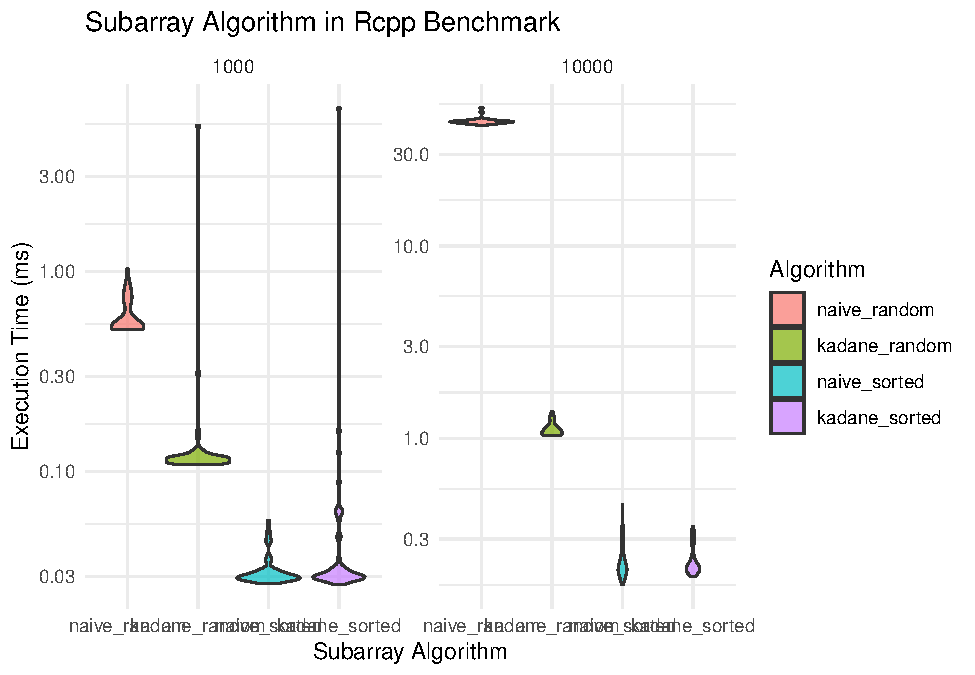
\includegraphics{MaxSubarray1D_files/figure-latex/benchmark2-1.pdf}

\begin{verbatim}
## # A tibble: 12 x 9
##        n case            algo       min       q1  median    mean      q3     max
##    <dbl> <fct>           <fct>    <dbl>    <dbl>   <dbl>   <dbl>   <dbl>   <dbl>
##  1  1000 mostly_negative Naif    0.261   0.262    0.267  3.18e-1 3.08e-1  0.871 
##  2  1000 mostly_negative Kadane  0.003   0.0031   0.0034 6.00e-3 6.78e-3  0.0278
##  3  1000 mostly_positive Naif    0.260   0.261    0.262  2.68e-1 2.72e-1  0.299 
##  4  1000 mostly_positive Kadane  0.0025  0.0026   0.0027 3.53e-3 3.1 e-3  0.0272
##  5  1000 random          Naif    0.260   0.261    0.262  2.72e-1 2.64e-1  0.428 
##  6  1000 random          Kadane  0.0028  0.00292  0.0031 4.39e-3 3.8 e-3  0.0411
##  7 10000 mostly_negative Naif   25.7    26.2     26.6    2.68e+1 2.71e+1 28.3   
##  8 10000 mostly_negative Kadane  0.026   0.0273   0.0340 3.40e-2 3.83e-2  0.0667
##  9 10000 mostly_positive Naif   25.8    26.5     27.0    2.69e+1 2.72e+1 29.2   
## 10 10000 mostly_positive Kadane  0.0211  0.0221   0.0272 3.07e-2 3.67e-2  0.078 
## 11 10000 random          Naif   25.9    26.4     26.6    2.68e+1 2.71e+1 28.4   
## 12 10000 random          Kadane  0.0274  0.0410   0.0511 5.16e-2 6.28e-2  0.0891
\end{verbatim}

\begin{Shaded}
\begin{Highlighting}[]
\FunctionTok{library}\NormalTok{(dplyr)}
\FunctionTok{library}\NormalTok{(tidyr)}

\NormalTok{gain\_comparison }\OtherTok{\textless{}{-}}\NormalTok{ stats\_results }\SpecialCharTok{\%\textgreater{}\%}
  \FunctionTok{group\_by}\NormalTok{(n, case) }\SpecialCharTok{\%\textgreater{}\%}
  \FunctionTok{summarise}\NormalTok{(}
    \AttributeTok{gain =}\NormalTok{ median[algo }\SpecialCharTok{==} \StringTok{"Naif"}\NormalTok{]}\SpecialCharTok{/}\NormalTok{median[algo }\SpecialCharTok{==} \StringTok{"Kadane"}\NormalTok{],}
    \AttributeTok{.groups =} \StringTok{"drop"}
\NormalTok{  )}

\FunctionTok{print}\NormalTok{(gain\_comparison)}
\end{Highlighting}
\end{Shaded}

\begin{verbatim}
## # A tibble: 6 x 3
##       n case             gain
##   <dbl> <fct>           <dbl>
## 1  1000 mostly_negative  78.6
## 2  1000 mostly_positive  97.1
## 3  1000 random           84.4
## 4 10000 mostly_negative 782. 
## 5 10000 mostly_positive 992. 
## 6 10000 random          520.
\end{verbatim}

\begin{Shaded}
\begin{Highlighting}[]
\NormalTok{gain\_plot }\OtherTok{\textless{}{-}}\NormalTok{ gain\_comparison }\SpecialCharTok{\%\textgreater{}\%}
  \FunctionTok{ggplot}\NormalTok{(}\FunctionTok{aes}\NormalTok{(}\AttributeTok{x =}\NormalTok{ case, }\AttributeTok{y =}\NormalTok{ gain, }\AttributeTok{fill =} \FunctionTok{factor}\NormalTok{(n))) }\SpecialCharTok{+}
  \FunctionTok{geom\_col}\NormalTok{(}\AttributeTok{position =} \FunctionTok{position\_dodge}\NormalTok{(}\AttributeTok{preserve =} \StringTok{"single"}\NormalTok{)) }\SpecialCharTok{+}
  \FunctionTok{geom\_text}\NormalTok{(}\FunctionTok{aes}\NormalTok{(}\AttributeTok{label =} \FunctionTok{round}\NormalTok{(gain, }\DecValTok{1}\NormalTok{)), }
            \AttributeTok{position =} \FunctionTok{position\_dodge}\NormalTok{(}\AttributeTok{width =} \FloatTok{0.9}\NormalTok{),}
            \AttributeTok{vjust =} \SpecialCharTok{{-}}\FloatTok{0.5}\NormalTok{) }\SpecialCharTok{+}
  \FunctionTok{labs}\NormalTok{(}
    \AttributeTok{title =} \StringTok{"Gain de performance de Kadane vs Naïf"}\NormalTok{,}
    \AttributeTok{x =} \StringTok{"Type de données"}\NormalTok{,}
    \AttributeTok{y =} \StringTok{"Facteur d\textquotesingle{}accélération"}\NormalTok{,}
    \AttributeTok{fill =} \StringTok{"Taille (n)"}
\NormalTok{  ) }\SpecialCharTok{+}
  \FunctionTok{theme\_minimal}\NormalTok{() }\SpecialCharTok{+}
  \FunctionTok{scale\_fill\_brewer}\NormalTok{(}\AttributeTok{palette =} \StringTok{"Pastel1"}\NormalTok{)}

\FunctionTok{print}\NormalTok{(gain\_plot)}
\end{Highlighting}
\end{Shaded}

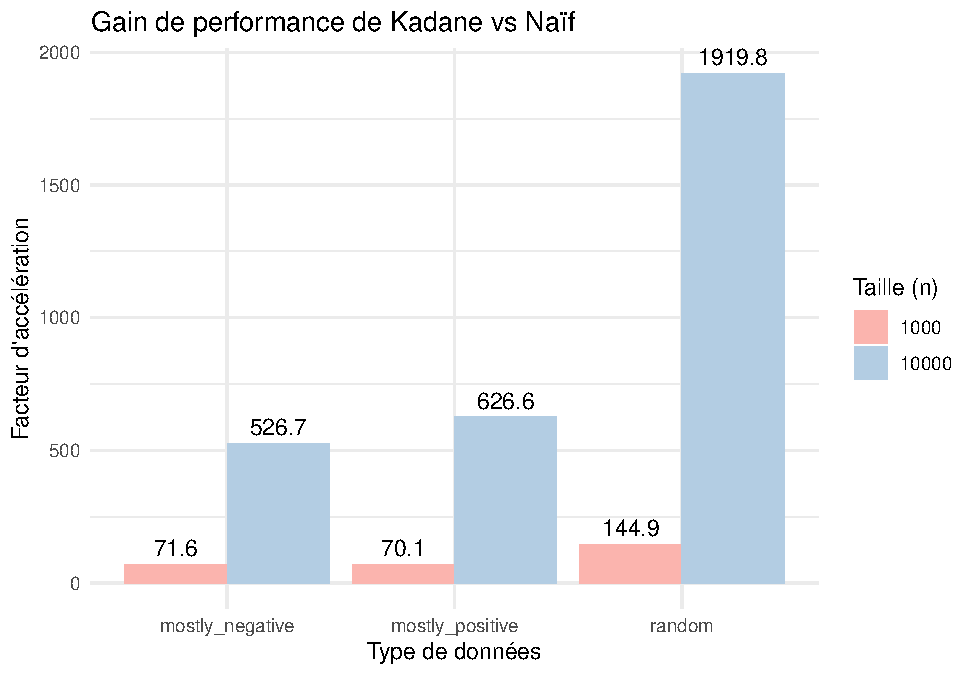
\includegraphics{MaxSubarray1D_files/figure-latex/unnamed-chunk-16-1.pdf}

Ces résultats montrent que les algorithmes sont plus efficaces sur des
données avec une structure, comme celles qui sont majoritairement
positives ou négatives, par rapport aux données complètement aléatoires.

\end{document}
